\documentclass[kravspec/krav.tex]{subfiles}

\begin{document}
\section{Kommunikationsmodul}

\section{Styrmodul}
\begin{figure}[h]
    \centering
    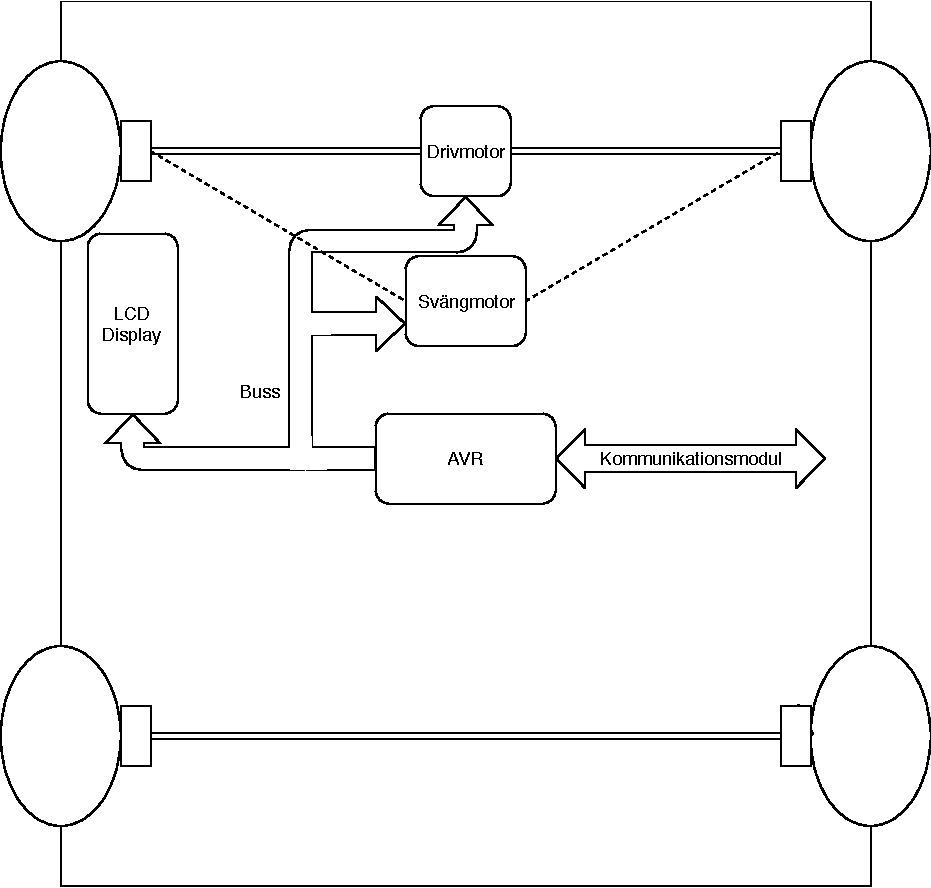
\includegraphics[width=0.6\linewidth]{kravspec/figures/styrmodul.pdf}
    \caption{Styrmodul}
    \label{fig:styrmodul}
\end{figure}

\section{Sensormodul}
\subsection{Beskrivning}
Sensormodulen består av enhetens alla sensorer och en microprocessor. Dess
uppgift är att hantera information från de olika sensorerna och även
ut
\subsection{Gränssnitt}
\subsection{Krav}

\end{document}
